\section{Introduction}
\label{sec:intro}

Social Event Detection (SED) organizes high-velocity streams of short, noisy social-media posts into coherent real-world incidents as stories unfold~\citep{mcminn2013building,mazoyer2020french}. Recent systems span incremental heterogeneous Graph Neural Networks (GNNs)~\citep{cao2021kpgnn}, unsupervised 2-dimensional Structural Entropy (2D-SE) minimization~\citep{cao2024hisevent}, hyperbolic relational encoders~\citep{li2024rplmsed,yu2025hypersed}, and Large Language Model (LLM) augmentation~\citep{qiu2025lsed,qiu2026lhg,liu2026ragsede}. Although LLMs readily resolve slang, implicit event co-reference, and subtle narrative shifts, querying an LLM on every incoming tweet is cost- and latency-prohibitive. Operational streaming pipelines therefore operate under tight token budgets where only roughly $1\%$ or fewer of arriving messages can trigger an LLM API call ($\sim 10\text{k}$ total input and output tokens per daily block).

In this strictly budgeted regime, existing active querying strategies fall prey to what we term the \textbf{Single-Post Fallacy}. Even when a selector carefully picks informative individual tweets---such as Representativeness-plus-Diversity Maximal Marginal Relevance (MMR) sampling~\citep{liu2026ragsede,carbonell1998mmr}---or uncertain post pairs---such as Cequel-style must-link/cannot-link edge queries~\citep{wang2025cequel}---each $500$-token LLM decision touches only $1$--$2$ messages directly. Under a $10\text{k}$-token daily cap across $2{,}000$--$4{,}800$ arriving posts, an 8B model can afford roughly $10$--$25$ calls per day. Our controlled bilingual experiments confirm that \texttt{Random}, \texttt{Rep-Div}, and \texttt{Cequel-Edge} achieve near-zero stream-wide AMI movement ($-0.0014$ to $+0.0001$), and even propagating pairwise decisions via cluster-level transitive closure (\texttt{Cequel-Transitive}) triggers over-merging chains that push Event Macro-$B^3$ \emph{below} the unsupervised initialization. Simply spending fewer tokens on isolated tweets fails to reshape the global partition.

To understand how finite LLM judgments \emph{can} produce stream-wide gains without future information or metric inflation, we perform a granular diagnostic audit (Stage~1) on unsupervised fixed-point 2D-SE partitions~\citep{li2016structural,cao2024hisevent} across English (\texttt{Event2012}~\citep{mcminn2013building}) and French (\texttt{Event2018}~\citep{mazoyer2020french}) streams. Four empirical findings govern the problem geometry:
\begin{enumerate}
    \item \textbf{Severe False-Split Dominance ($11.6\times$--$44.6\times$):} Across unseen held-out blocks, pairwise False Splits outnumber False Merges by $44.64\times$ on \texttt{Event2012} ($11.60\times$ on development blocks) and $11.59\times$ on \texttt{Event2018} ($14.89\times$ on dev), shattering evolving stories across hashtag and phrasing variants.
    \item \textbf{Zero-Boundary-Entropy Impure Interiors:} False Merges rarely form balanced $50/50$ cuts. On held-out streams, $36.2\%$ (EN) and $16.2\%$ (FR) of nodes exhibit zero inter-community boundary entropy, while impure super-clusters ($|C|\ge 10$, purity $<0.90$, accounting for $21.1\%$ EN and $26.5\%$ FR clusters) trap secondary incidents at a median minority share of $0.231$ (EN) and $0.233$ (FR)---with over half ($56.4\%$ / $54.2\%$) concentrated in $[0.10, 0.25]$. Traditional boundary-uncertainty routers miss these interiors completely, whereas balanced spectral Fiedler cuts~\citep{fiedler1973algebraic} bisect the dominant event.
    \item \textbf{Transparent Unqueried Leverage Accounting:} Because each mesoscopic prompt shows up to $6$ central medoid tweets ($3$ per side), counting only $1$--$2$ ``primary'' nodes per call leaks shown medoids into the ostensibly ``unqueried'' evaluation set $U_t$. We strictly mask \emph{all} prompt-shown medoids ($1.79\%$--$3.87\%$ total block exposure) out of $U_t$ so reported propagation gains reflect genuine unshown-post restructuring.
    \item \textbf{The Cross-Day Prototype Precision-Recall Trap:} Multi-day event recurrence reaches $55.67\%$ (EN) and $62.05\%$ (FR) on held-out blocks. Unsupervised cosine linking raises Micro-$B^3$ yet causes cross-story over-merges that degrade Global Macro-$B^3$; meanwhile, an overly low fallback threshold ($\tau_{\text{fb}}=0.72$) or miscalibrated ambiguity band ($[0.55, 0.80)$) lets a strong unsupervised prototype threshold ($\tau=0.80$) beat naive cross-day LLM gating.
\end{enumerate}

We address these bottlenecks with \textbf{SUG-Meso} and \textbf{SUG-CrossLLM-v2} (Figure~\ref{fig:overview}). Within each block, \textbf{SUG-Meso} interleaves inter-cluster \texttt{MERGE\_PAIR} candidates with minority-pocket \texttt{SPLIT\_SEAM} candidates extracted by deterministic farthest-point spherical $k$-means~\citep{gonzalez1985clustering,banerjee2005clustering} and regularized by non-entity cut divergence, under strictly zero-lookahead causal token budgets (\texttt{CausalUniform} Fixed/Carryover and \texttt{CausalSliding}). Across blocks, \textbf{SUG-CrossLLM-v2} links high-confidence matches ($\ge 0.85$) at zero token cost and deploys precision-calibrated LLM verification inside $[0.65, 0.85)$ with fallback $\tau_{\text{fb}}=0.85$. Guided by a \textbf{Candidate Base-Rate $\times$ Prompt Framing} principle calibrated strictly on dev blocks, we pair high-prior within-block seams with \texttt{Action-First} prompts and low-prior cross-day candidates with \texttt{Extract-Then-Compare} prompts.

\begin{figure*}[t]
  \centering
  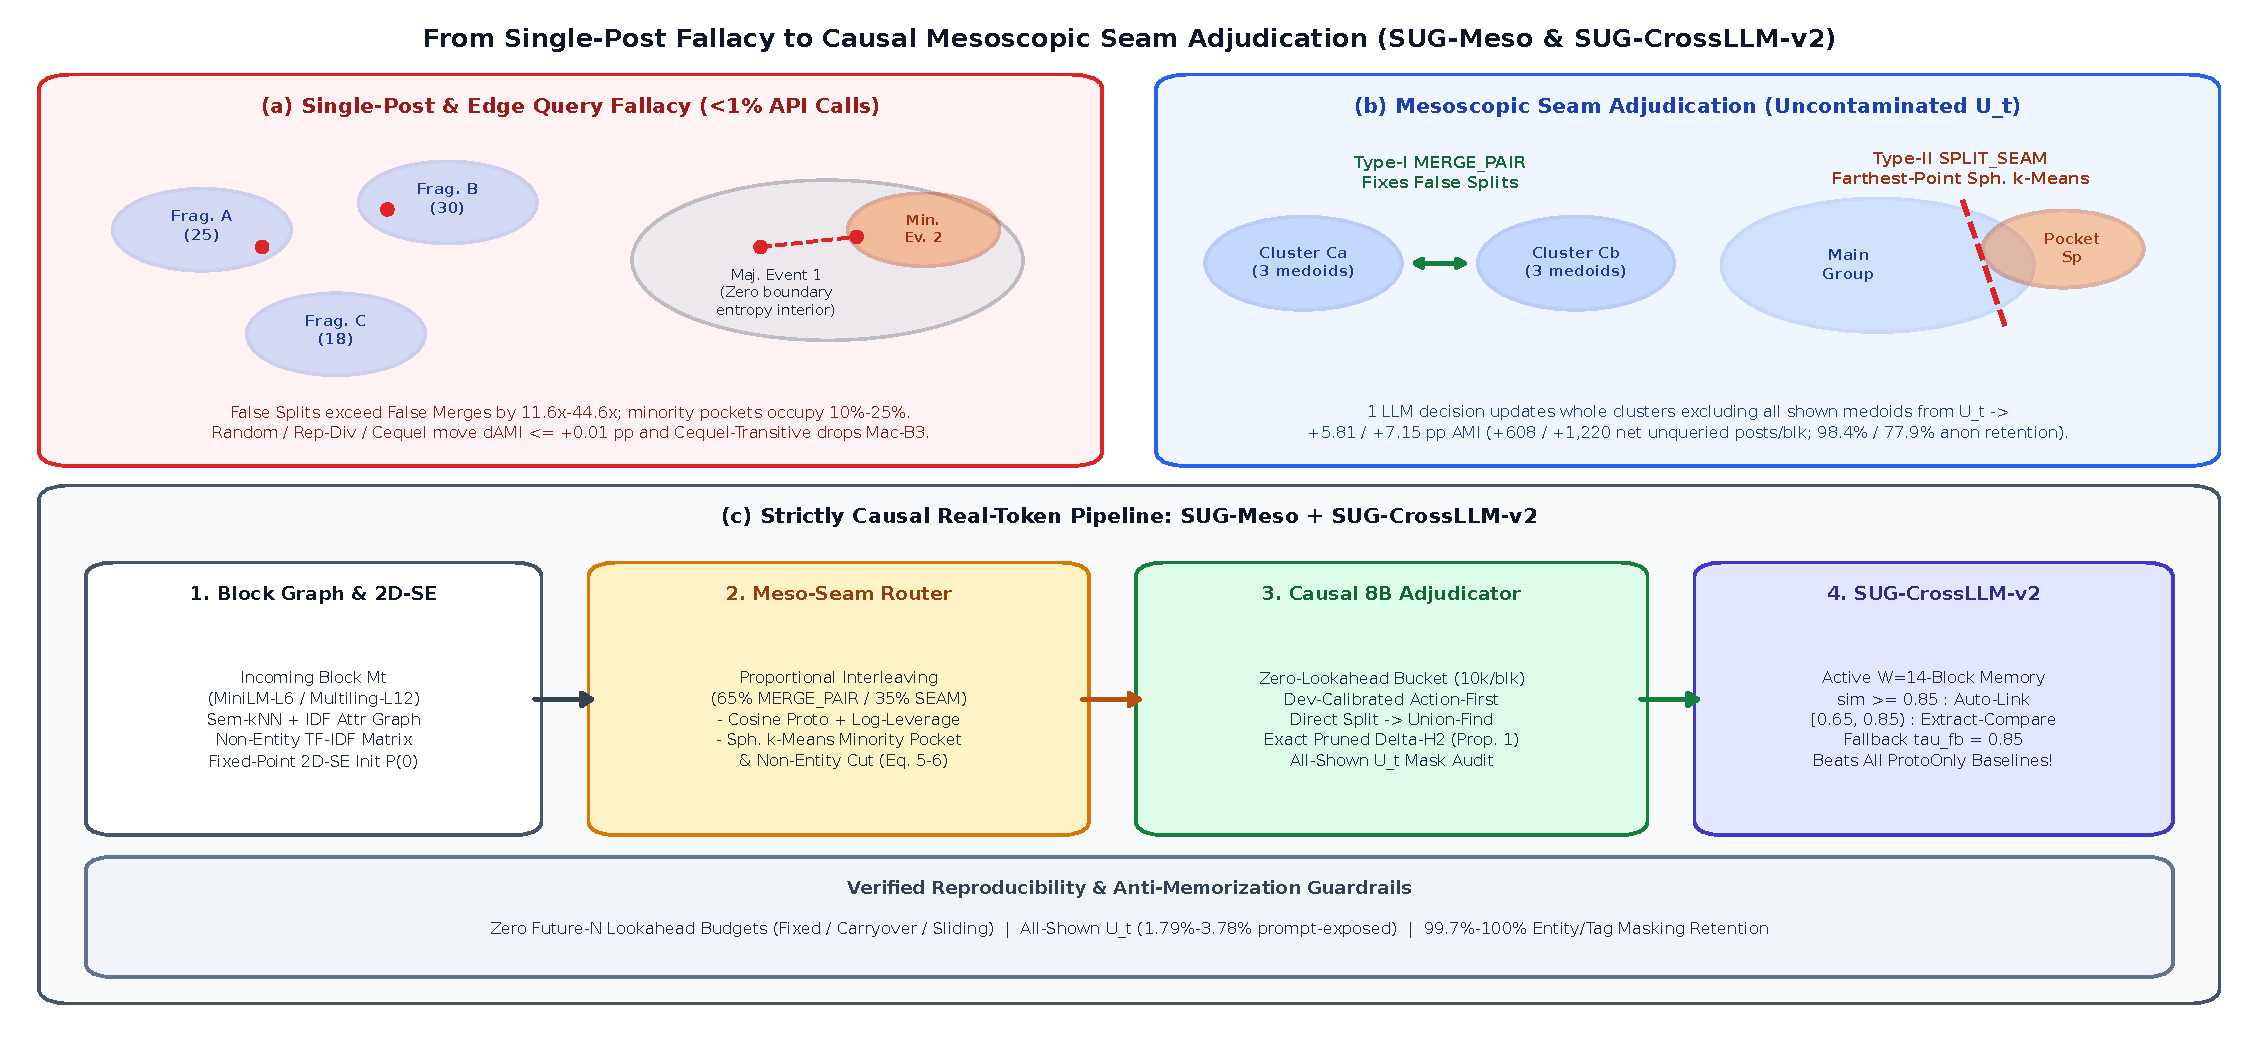
\includegraphics[width=\textwidth]{figures/fig_overview.pdf}
  \caption{Overview of the single-post fallacy versus strictly causal mesoscopic seam adjudication. (a)~Post- and edge-level selectors touch $1$--$2$ nodes per call while missing $11.6\times$--$44.6\times$ dominant false splits and zero-boundary-entropy minority pockets ($10\%$--$25\%$ share). (b)~\textbf{SUG-Meso} resolves whole fragmented cluster pairs and minority pockets while strictly excluding all prompt-shown medoids from the uncontaminated unqueried set $U_t$. (c)~The zero-lookahead streaming architecture combines fixed-point 2D-SE, symmetric seam routing, Dev-calibrated \texttt{Action-First} edits backed by Proposition~\ref{prop:exact_prune}, longitudinal \textbf{SUG-CrossLLM-v2}, and verified anti-memorization robustness.}
  \label{fig:overview}
\end{figure*}

Our contributions are fivefold:
\begin{itemize}
    \item \textbf{Diagnostic Reframing \& Uncontaminated Auditing:} We formalize strictly causal zero-lookahead real-token budgets alongside an uncontaminated \texttt{all\_shown} unqueried set $U_t$, quantifying exact False-Split asymmetries and minority-pocket geometries on bilingual streams.
    \item \textbf{Mesoscopic Intra- \& Cross-Block Framework (\texttt{SUG-Meso} \& \texttt{SUG-CrossLLM-v2}):} We unify prototype-leveraged cluster merges, deterministic farthest-point spherical $k$-means pocket splits, base-rate-calibrated prompting, and ambiguity-banded $[0.65, 0.85)$ longitudinal tracking.
    \item \textbf{Exact Full-Volume 2D-SE Theory:} Proposition~\ref{prop:exact_prune} derives exact graph- and cluster-volume shrinkage under edge pruning, proving an unconditional no-false-merge guarantee that corrects fixed-volume approximations ($+0.164160\text{ bit}$ on a canonical $3$-clique check).
    \item \textbf{Rigorous Causal Held-Out Benchmark \& Ablations:} Evaluated on $27$ unseen blocks ($65{,}856$ tweets) using \texttt{Qwen/Qwen3-8B}, \texttt{SUG-Meso} reaches $0.8976$ AMI ($+5.81\text{ pp}$) on \texttt{Event2012} and $0.8349$ AMI ($+7.15\text{ pp}$) on \texttt{Event2018}, significantly outperforming zero-LLM heuristics, \texttt{Cequel-Transitive}, multi-seed \texttt{Random}, and \texttt{Random-Meso} under Holm-corrected Wilcoxon tests, while \texttt{SUG-CrossLLM-v2} beats every unsupervised prototype threshold. Fine-grained Eq.~(5)/(6) ablations further reveal that relaxing the hard $\text{cond} \le 0.50$ filter unlocks an additional $+1.22$/$+1.23\text{ pp}$ Macro-$B^3$ and $+2.70$/$+4.34\text{ pp}$ Tail-$B^3$.
    \item \textbf{Anti-Memorization Verification:} A $27$-block anonymization stress test masking $99.7\%$--$100\%$ named entities, $100\%$ hashtags, and $100\%$ years yields $0\%$ true historical entity reconstruction while retaining $98.4\%$ (EN) and $77.9\%$ (FR) of AMI gains under pseudonymized co-reference, contrasting sharply with blind entity redaction to prove structural-semantic rather than memorization-driven gains.
\end{itemize}
